% NÃO altere as predefinições desse template!

\documentclass{ceel}

% ===========================
%Coloque aqui pacotes adicionais, se necessário
\usepackage{verbatim}
\usepackage{hyperref}

%%===========================

% Dados do trabalho
\title{}

% Autores: o primeiro será, necessariamente, o apresentador do trabalho
% Caso o trabalho não tenha 8 autores, exclua os campos que não foram preenchidos
\author[1]{\underline{Lesly Viviane Montúfar Berrios}\thanks{leslymontufar@ufu.br}}
\author[1]{Segundo Autor}



% Adicione as instituições de cada autor e indique corretamente no campo acima
\affil[1]{FEELT - Universidade Federal de Uberlândia}

\begin{document}

\inserirtitulo

\begin{multicols}{2}

% Adicione o Resumo do seu trabalho no campo abaixo, com início em "O objetivo [...]"
\textbf{\emph{Resumo} - O objetivo deste documento é instruir os autores sobre a preparação de artigos para submissão e publicação nos anais da XVII Conferência de Estudos em Engenharia Elétrica. Os autores deverão utilizar estas normas desde a elaboração da versão inicial até a versão final de seus trabalhos. Somente os artigos que estejam integralmente de acordo com estas normas serão aceitos para publicação.}
\vspace*{10pt}

%Adicione as palabras-chave do seu trabalho abaixo
\textbf{\emph{Palavras-Chave}- Os autores devem apresentar um conjunto de no máximo 6 palavras-chave (em ordem alfabética) que possam identificar os principais tópicos abordados no trabalho.}


\begin{center}
%Insira aqui o Título do trabalho em inglês
\noindent\textbf{\large \uppercase{TITLE HERE IN ENGLISH IS MANDATORY}}
\end{center}

%Insira aqui o resumo do seu trabalho em inglês
\textbf{\emph{Abstract} - The objective of this document is to instruct the authors on the preparation of papers for submission and publication in proceedings of XVII Conference of Studies in Electrical Engineering. The authors should use these guidelines since the establishment of the initial version to the final version of their works. Only papers that are integrally in accordance with these norms will be accepted for publication. }
\vspace*{10pt}

%Insira aqui as palavras-chave do seu trabalho em inglês
\textbf{\emph{Keywords} - Authors shall provide a maximum of 6 keywords (in alphabetical order) in order to identify the major topics of the paper.}


\begin{center}
%Insira a nomenclatura que você deseja listar para uso em seu trabalho
\uppercase{NOMENCLATURA (EXEMPLOS - OPCIONAL)}
\end{center}
\begin{itemize}
\setlength\itemsep{1mm}
\item [$P$] Número de par de pólos.
\item [$V_{qd}$] Componentes da tensão de estator.
\item [$I_{qd}$] Componentes da corrente de estator.
\end{itemize}

%Introdução: Caso queira pode mudar o título da seção para qualquer outro. Dentro das chaves insira o título da seção e abaixo insira o texto da mesma.
\section{Introdução}

\begin{comment}
Serão aceitos trabalhos em português e também em inglês, desde que estes últimos também atendam a estas normas. Os textos submetidos em português devem conter adicionalmente o título (title), o resumo (abstract) e as palavras-chave (keywords) em inglês, obrigatoriamente.

Caso seja pertinente, pode ser incluída imediatamente antes da introdução uma nomenclatura das variáveis utilizadas no texto. Este item não deve levar numeração de referência, assim como os itens agradecimentos, referências bibliográficas e dados biográficos.

A introdução tem o objetivo geral de apresentar a natureza do problema enfocado no trabalho, através de adequada revisão bibliográfica, o propósito e a contribuição do artigo submetido.

Os anais da XVII CEEL - Conferência de Estudos em Engenharia Elétrica - representam um meio apropriado onde pesquisadores atuantes nas diversas áreas que englobam Engenharia Elétrica e Engenharia Biomédica podem apresentar e discutir suas atividades e contribuições científicas. Neste contexto, o Comitê Responsável pela Submissão dos Artigos convida os interessados a apresentarem artigos completos que envolvam o “estado da arte”, por meio de resultados teóricos e experimentais, além de informações tutorais, nos tópicos de interesse de profissionais, pesquisadores, educadores e estudantes de Engenharia Elétrica, Engenharia Biomédica e áreas afins. 

Caso o trabalho, ou parte dele, já tenha sido apresentado e publicado em alguma revista ou conferência, nacional ou internacional, deve ser anexada no corpo do trabalho declaração dos autores com estas informações (quando e onde). Por outro lado, caso este nunca tenha sido publicado na sua totalidade, não há necessidade desta declaração.

Os trabalhos somente serão aceitos através de submissão eletrônica. Os autores deverão submeter e acompanhar todo o processo de suas contribuições através da página da XVII CEEL, cujo endereço é: \url{http://www.peteletricaufu.com/ceel}.

%Formatação Geral: Caso queira pode mudar o título da seção para qualquer outro. Dentro das chaves insira o título da seção e abaixo insira o texto da mesma.
\section{Formatação Geral}
Como já salientado, cabe(m) ao(s) autor(es) do trabalho a preparação dos originais de acordo com estas normas de edição e, posteriormente, seu envio de forma eletrônica, através do site \url{www.peteletricaufu.com/ceel}. Os trabalhos que estiverem fora dos padrões estabelecidos serão recusados, com a devida informação ao(s) autor(es) correspondente(s).

A Comissão Editorial não assumirá qualquer responsabilidade quanto a correções, e possíveis erros da reprodução dos originais para publicação.

%Apresentação do Texto: Caso queira pode mudar o título da seção para qualquer outro. Dentro das chaves insira o título da seção e abaixo insira o texto da mesma.
\subsection{Apresentação do Texto}
O artigo completo deve conter no mínimo 4 (quatro) e no máximo 6 (seis) páginas. Não serão aceitos trabalhos que estejam fora desses limites em nenhuma hipótese. 

Na formatação das páginas, as margens superior e inferior deverão ser fixadas em 25 mm, a margem esquerda em 18 mm e a margem direita em 12 mm. As colunas de textos deverão apresentar uma largura igual a 87 mm e um espaçamento entre si de 6 mm.

Devem-se usar, obrigatoriamente, as unidades do Sistema Internacional (SI ou MKS).

%Edição do texto: Caso queira pode mudar o título da seção para qualquer outro. Dentro das chaves insira o título da seção e abaixo insira o texto da mesma.
\subsection{Edição do Texto}
A editoração do trabalho deve ser feita selecionando o formato A4 ($297$mm $\times$ $210$mm).

Como processador de texto, estimula-se o uso do processador Word for Windows. 

O espaçamento entre linhas deve ser simples, e a cada título ou subtítulo, deve-se deixar uma linha em branco.


\begin{enumerate}[1)]
\item \emph{Tamanhos e tipos de letras}\\
Os tamanhos das letras especificadas nesta norma seguem o padrão do processador Word for Windows e o tipo de letra utilizado é Times New Roman. A Tabela I mostra os tamanhos padrões de letras utilizadas nas diversas partes deste artigo. 

\begin{minipage}[h]{\columnwidth}
\begin{scriptsize}
\captionsetup{type=table}
\caption{Tamanhos e tipos de letras utilizadas no texto}
\begin{tabular}{p{1cm}p{1.8cm}p{1.8cm}p{1.8cm}}\hline
\textbf{Tamanho (pontos)}&	\textbf{Normal}&\textbf{Negrito} & \textbf{Negrito Itálico} \\\hline
8 & Texto de tabelas &  &  \\ \hline
9 & Legendas de figuras, legendas de tabelas & & \\\hline
10 & Instituição dos autores, texto em geral & Texto do resumo e palavras-chave; títulos de seções primárias &  Título do resumo e palavras-chave; títulos de seções secundárias.\\\hline
12 & Nomes dos autores & Título em inglês &  \\\hline
14 &  & Título do trabalho &  \\\hline
\end{tabular}
\end{scriptsize}
\end{minipage}
\item \emph{Tabulação dos parágrafos}\\
A tabulação a ser utilizada na primeira linha de cada parágrafo deverá ser fixada em 4 mm.
\end{enumerate}

\subsection{Organização das Seções}
A organização do trabalho em títulos e subtítulos serve para dividi-lo em seções, que ajuda o leitor a encontrar determinados assuntos de interesse dentro do trabalho. Também auxiliam os autores a desenvolverem de forma ordenada seu trabalho. Os títulos devem ser organizados em seções primárias, secundárias e terciárias.

As seções primárias são os títulos de seções propriamente ditos, sendo grafadas em letras maiúsculas, em negrito, centradas na coluna, separadas por uma linha em branco anterior e uma posterior, e utilizam numeração romana e sequencial.

As seções secundárias são os subtítulos das seções primárias. Apenas a primeira letra das palavras que a compõe, são grafadas em letra maiúscula, na margem esquerda da coluna sendo separada do resto do texto por uma linha em branco anterior. A designação das seções secundárias é feita com letras maiúsculas, seguidas de um ponto, utilizando grafia em itálico e em negrito.

As seções terciárias são subdivisões das seções secundárias. Apenas a primeira letra da primeira palavra que a compõe é grafada em letra maiúscula, seguindo o espaçamento dos parágrafos. A designação das seções terciárias é feita com algarismos arábicos, seguidos de um parêntese, utilizando grafia em itálico (sem negrito).
\section{Composição do artigo}
Nesta seção são apresentados os principais estilos utilizados para edição do trabalho em forma de artigo.
\subsection{Organização Geral}
Os artigos a serem publicados em Português nos anais da XVII CEEL devem conter 8 partes principais: 1) Título; 2) Autores e suas instituições de origem; 3) Resumo e Palavras-Chave; 4) Título em inglês (Title), Abstract e Keywords; 5) Introdução; 6) Corpo do trabalho; 7) Conclusões; 8) Referências. 

Já os artigos a serem publicados em Inglês devem compreender 7 partes principais: 1) Título em inglês (Title); 2) Autores e suas instituições de origem; 3) Abstract e Keywords; 4) Introduction; 5) Corpo do trabalho em inglês; 6) Conclusions; 7) References. 

A ordem citada acima deve ser respeitada, a menos que os autores usem alguns itens adicionais, a saber: Nomenclatura (Terminology), Agradecimentos (Acknowledgements), Dados Biográficos (Biographical Data) e Apêndices (Appendices). Ver as normas específicas na seção V. 

A seguir serão feitos alguns comentários sobre os principais itens acima.
\begin{enumerate}[1)]
\item \emph{Título}\\
O título do trabalho deve ser o mais sucinto possível, indicando claramente o assunto de que se trata. Deve estar centrado no topo da primeira página, sendo impresso em negrito, tamanho 14 pontos, com todas as letras em maiúsculo.
\item \emph{Autores e instituições de origem}\\
Abaixo do título do trabalho, também centrados na página, devem ser informados os nomes dos autores e da(s) instituição(ões) a que pertencem. Poderão ser abreviados os nomes e sobrenomes intermediários e escritos na sua forma completa o primeiro nome e o último sobrenome (letras do tipo 12 pontos). Imediatamente abaixo do nome dos autores, informar as instituições a que pertencem e os endereços completos (letras do tipo 10 pontos).
\item \textit{Resumo e palavras-chave}\\
Resumo é considerado como uma das partes mais importantes do trabalho. É baseado nas informações contidas neste resumo que os trabalhos técnicos são indexados e armazenados em bancos de dados. Este resumo deve conter no máximo 200 palavras de forma a indicar as idéias principais apresentadas no texto, procedimentos e resultados obtidos. O resumo não deve ser confundido com uma introdução do trabalho e muito menos conter abreviações, referências bibliográficas, figuras, etc. Na elaboração deste resumo, como também em todo o trabalho, deve ser utilizada a forma impessoal como, por exemplo, “... Os resultados experimentais mostraram que...” ao invés de “... os resultados que nós obtivemos mostraram que...”. A palavra Resumo deve ser grafada em estilo itálico e em negrito. Já o texto deste Resumo será em estilo normal e em negrito.\\

Palavras-Chave são termos para indexação que possam identificar os principais tópicos abordados no trabalho. O termo Palavras-Chave deve ser grafado em estilo itálico e em negrito. Já o texto deste item será em estilo normal e em negrito.
\item \emph{Título, resumo e palavras-chave em inglês}\\
Esta parte é obrigatória somente para artigos redigidos em português. O título em português deverá ser reproduzido em inglês, conforme normas apresentadas, destacando-se o estilo em letras todas maiúsculas, negrito e tamanho 12. 
O termo Abstract (resumo em inglês) deve ser grafado em estilo itálico e em negrito. Já o texto deste Abstract (em inglês) será em estilo normal e em negrito. 
Keywords (palavras-chave em inglês) são termos para indexação, em inglês, que possam identificar os principais tópicos abordados no trabalho. O termo Keywords deve ser grafado em estilo itálico e em negrito. Já o texto deste item será em estilo normal e em negrito.
\item \emph{Introdução}\\
A introdução deve preparar o leitor para o trabalho propriamente dito, dando uma visão histórica do assunto, e servir como um guia a respeito de como o trabalho está organizado, enfatizando quais são as reais contribuições do mesmo em relação aos já apresentados na literatura. A introdução não deve ser uma repetição do Resumo, e deve ser a primeira seção do trabalho a ser numerada.
\item \emph{Corpo do trabalho}\\
Os autores devem organizar o corpo do trabalho em diversas seções, as quais devem conter de forma clara, as informações a respeito do trabalho desenvolvido, facilitando a compreensão do mesmo por parte dos leitores.
\item \emph{Conclusões}\\
As conclusões devem ser as mais claras possíveis, informando aos leitores sobre a importância do trabalho dentro do contexto em que se situa. As vantagens e desvantagens deste trabalho em relação aos já existentes na literatura devem ser comentadas, assim como os resultados obtidos, as possíveis aplicações práticas e recomendações de pesquisas futuras. Como regra geral, as conclusões devem vir logo após o corpo do trabalho e imediatamente antes das referências bibliográficas.
\item \emph{Referências}\\
As citações das referências bibliográficas ao longo do texto devem aparecer entre colchetes, antes da pontuação das sentenças nas quais estiverem inseridas. Devem ser utilizados somente os números das referências bibliográficas, evitando-se uso de citações do tipo “... conforme referência [2]...”.
O trabalho que foi aceito para publicação, mas que ainda não foi publicado, deve ser colocado nas referências bibliográficas com a citação “ainda não publicado”.
Os artigos de periódicos e anais devem ser incluídos iniciando-se pelos nomes dos autores (sobrenome, iniciais), seguido do título do trabalho, onde foi publicado (em itálico), número do volume, páginas, mês e ano da publicação. 
No caso de livros, após os autores (sobrenome, iniciais), o título deve ser em itálico, seguido da editora, da edição e do local e ano de publicação. 
No final destas normas, são mostrados alguns exemplos de como devem ser inseridas as referências bibliográficas.
\end{enumerate}
\section{Normas especiais}
Figuras, tabelas, equações e abreviações devem obedecer às normas apresentadas a seguir.
\subsection{Figuras e Tabelas}
As tabelas e figuras (desenhos ou reproduções fotográficas) devem ser intercaladas no texto logo após serem citadas pela primeira vez, desde que caibam dentro dos limites da coluna; caso necessário, utilizar toda a área útil da página. Quanto a legenda, esta deve ser situada acima da tabela (vide Tabela I) e abaixo da figura (vide Figura 1).

As tabelas devem possuir títulos e são designadas pela palavra Tabela, sendo numeradas em algarismos romanos, sequencialmente, conforme mostra a Tabela I.

As figuras necessitam de título, legenda, e são designadas pela palavra Figura no texto, numeradas em algarismos arábicos, sequencialmente, conforme mostra a Figura 1. A designação das partes de uma figura é feita pelo acréscimo de letras minúsculas ao número da figura, separadas por ponto, começando pela letra a, como por exemplo, Figura 1.a..

Com o intuito de facilitar a compreensão das figuras, a definição dos eixos das mesmas deve ser feita utilizando-se palavras (e não letras), exceto no caso de formas de onda e planos de fase. As unidades devem ser expressas entre parênteses. Por exemplo, utilize a denominação “Magnetização (A/m)”, ao invés de “M (A/m)”.

As figuras e tabelas devem ser centradas nas colunas, evitando posicioná-las entre as duas colunas. Na verdade, sugere-se evitar a utilização de tabelas e figuras, cujas dimensões ultrapassem as dimensões das colunas. O uso de tabelas e figuras de grandes dimensões é permitido somente quando for necessário para aumentar a nitidez das informações ali contidas.

\begin{minipage}[h]{\columnwidth}
\centering
\captionsetup{type=figure}
\caption{Curva de magnetização em função do campo aplicado.} 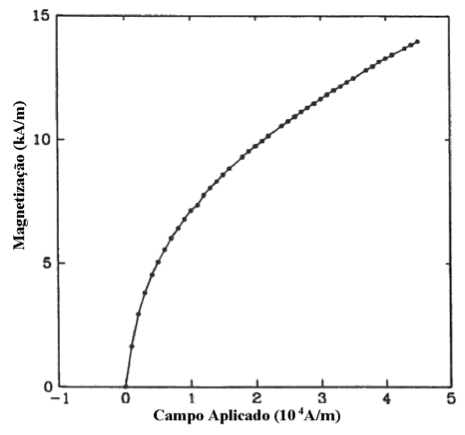
\includegraphics[scale=1]{figura}
\label{fig1}
\end{minipage}

\subsection{Equações}
A numeração das equações deve ser colocada entre parênteses, na margem direita, como no exemplo abaixo. As equações devem ser editadas de forma compacta, estar centralizadas na coluna e devem utilizar o estilo itálico. Caso a nomenclatura não seja inserida no início do texto, as grandezas devem ser definidas logo após as equações em que são indicadas.
\begin{equation}
\bigtriangleup I_L=I_0+\frac{\sqrt{3}}{2}\cdot\frac{V_i}{Z}
\end{equation}
Onde:\\

\begin{tabular}{lrl}
$\bigtriangleup I_L$ &-&Corrente de pico no indutor ressonante.\\
$I_0$&-&Corrente de carga.\\
$V_i$&-&Tensão de alimentação.\\
$Z$&-&Impedância característica do circuito ressonante.
\end{tabular}

\subsection{ Abreviações e Siglas}
As abreviações a serem utilizadas no texto, devem ser definidas na primeira vez em que aparecerem, como por exemplo, “... Modulação por Largura de Pulso (PWM)...”.
\section{NORMAS PARA SEÇÕES ADICIONAIS}

Caso sejam utilizadas seções adicionais opcionais como Nomenclatura; Agradecimentos, Dados Biográficos e Apêndices, as seguintes instruções devem ser observadas:
\subsection{Nomenclatura} 
A nomenclatura consiste na definição das grandezas e símbolos utilizados ao longo do trabalho. Caso seja incluído, este item não deve ser numerado e deve preceder o item Introdução. Caso os autores optem por não inserir este item, as definições das grandezas e símbolos utilizados devem ser incluídas ao longo do texto, logo após o seu aparecimento. No início destas normas é apresentado um exemplo para este item opcional.
\subsection{Agradecimentos}
Os agradecimentos a eventuais colaboradores não recebem numeração e devem ser colocadas no texto, antes das referências bibliográficas. No final deste trabalho é mostrado um exemplo de como podem ser feitos estes agradecimentos.
\subsection{Dados biográficos}
Os dados biográficos dos autores deverão estar na mesma ordem de autores colocados no início do trabalho e, caso sejam incluídos, deverão conter basicamente os seguintes dados:
\begin{itemize}
\item Nome Completo (em negrito e sublinhado);
\item	Local e ano de nascimento;
\item	Local e ano de Graduação e Pós-Graduação;
\item	Experiência Profissional (instituições e empresas onde trabalhou, número de patentes obtidas, áreas de atuação, atividades científicas relevantes, sociedades científicas a que pertence, etc.).
\end{itemize}
\subsection{Apêndices}
São materiais de importância secundária para compreensão do trabalho, mas que devem seguir a formatação geral dos textos do artigo sendo numerados em forma sequencial (Apêndice I, Apêndice II, etc.). Estes, quando incluídos, devem ocupar a parte final do artigo.\\

\textbf{OBSERVAÇÃO: }Quando do fechamento do artigo, o conteúdo da última página deve ser distribuído uniformemente utilizando ambas as colunas de tal forma que elas fiquem tão paralelas quanto possível (ver abaixo).
\end{comment}

\section{CONCLUSÕES}
Este artigo foi integralmente editado conforme as normas exigidas pela XVII Conferência de Estudos em Engenharia Elétrica. Portanto, este deve ser utilizado como template para o(s) autor(es) de trabalho(s) técnico-científico(s) redigir(em) seu(s) artigo(s) com a finalidade de submissão e publicação na XVII CEEL.

\begin{comment}
\section*{ AGRADECIMENTOS (OPCIONAL)}
Os autores agradecem a Fulano de Tal, pela colaboração neste trabalho. Este projeto foi financiado pelo CNPq (processo xxyyzz).
\end{comment}
%==================================
% REFERÊNCIAS
%==================================
\begin{thebibliography}{9} % apague as linhas abaixo e insira aqui bibliografia

\bibitem{leon-chua}	
    L. Chua,
    “Memristor-the missing circuit element”, 
    in \emph{IEEE Transactions on circuit theory}, VOL. CT-18, NO. 5, Setembro 1971.
   
\end{thebibliography}

\begin{comment}
\section*{DADOS BIOGRÁFICOS (OPCIONAL)}
\noindent \underline{\textbf{Leon Chua}}, nascido em 01/02/1980 em Uberlândia-MG, é engenheiro eletricista (2003), mestre (2005) e doutor em Engenharia Elétrica (2010) pela Universidade Federal de Uberlândia. De 2010 a 2014 foi coordenador do Laboratório de Eletrônica de Potência. Atualmente é professor titular da Universidade Federal de Uberlândia. Suas áreas de interesse são: Eletrônica de Potência, Qualidade do Processamento da Energia Elétrica, Sistemas de Controle Eletrônicos e Acionamentos de Máquinas Elétricas. É sócio efetivo da Sociedade Brasileira de Eletrônica de Potência (SOBRAEP) desde 2010.
\vspace{0.2cm}

\noindent \underline{\textbf{R.Stanley Williams}}, nascido em 01/02/1980 em Uberlândia-MG, é engenheiro eletricista (2003), mestre (2005) e doutor em Engenharia Elétrica (2010) pela Universidade Federal de Uberlândia. De 2010 a 2014 foi coordenador do Laboratório de Eletrônica de Potência. Atualmente é professor titular da Universidade Federal de Uberlândia. Suas áreas de interesse são: Eletrônica de Potência, Qualidade do Processamento da Energia Elétrica, Sistemas de Controle Eletrônicos e Acionamentos de Máquinas Elétricas. É sócio efetivo da Sociedade Brasileira de Eletrônica de Potência (SOBRAEP) desde 2010.

\end{comment}
%--- FIM ---



\end{multicols}
\end{document}
